\chapter{Current UCN Facility at TRIUMF}

% Based on simulations, a 40~$\mu$A of current produces a background of
% XXX mSev.

The current vertical UCN cryostat at TRIUMF is the same UCN cryostat
developed and tested at RCNP, Japan between 19xx and
2012(?)~\cite{masuda2002spallation,masuda2012spallation}.  In 2016,
the cryostat was shipped to triumf for further UCN experiments. These
experiments were essential for better understanding of the cryostat
and design of the next generation UCN source.  The vertical source was
modified to fulfill the safety requirements at TRIUMF (find where and
what those are.)  The current location of the vertical source is at
the meson hall experimental area.  A picture of the UCN facitity is
shown below.

The unique feature of the UCN source at TRIUMF is the combination of
spallation neutrons and superfluid helium for UCN production. This
will be discussed in detail in the following sections.
%%%%%%%%%%%%%%%%%%%%%%%%%%%%%

%%%%%%%%%%%%%%%%%%%%%%%%%%%%%
\section{UCN beamline}
%TRIUMF's proton beam is provided by a 520~Mev cyclotron.
TRIUMF produces negatively charged hydrogen ions from an ion
source. These ions are then accelerated in the 520~Mev cyclotron in an
outward spiral trajectory. A thin graphite stripper foil removes the
electrons from the hydrogen ion while protons can pass through. The
proton, because it is a positively charged particle, is deflected in
the outward direction due to the magnetic field and is directed to a
proton beam line. TRIUMF has four independent extraction probes with
various sizes of foils to provide protons simultaneously to up to four
beam lines.


The 120~$\mu$A beam (BL1A) enters the Meson Hall where the UCN
facility is located. The vertical UCN source was designed for a
maximum of 40~$\mu$A beam on target. As a result, only one third of
the beam can go to the UCN experimental area and the rest is shared
with different experimental facilities.

The microstructure of BL1A is in pulses with approximately 1~ms
periods of beam followed by a 50-100~$\mu$s periods of no beam.  This
is shown in Fig.~(\ref{fig:bl1u})~\cite{Nick_thesis}. A
kicker magnet kicks away 1/3 of the beam to BL1U. For most of the UCN
data taking, the beam was on for 1~min and off for 4~min. These times
are adjustable.

After the kicker magnet, the septum magnet bends the beam to the
target and the quadropoles focus the beam to the target.


\begin{figure}[h]
  \centering
  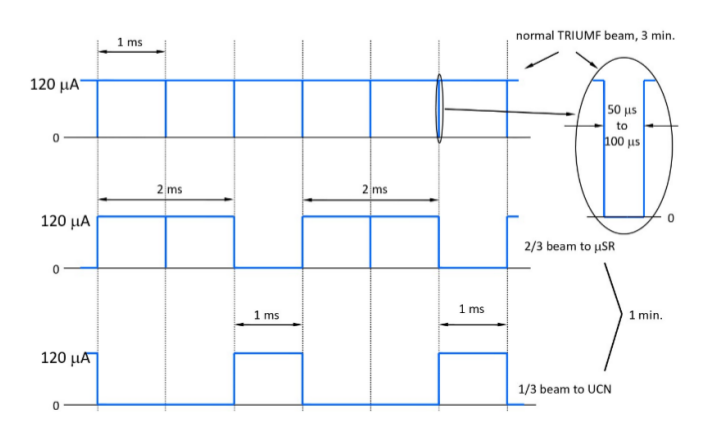
\includegraphics[width=0.9\textwidth]{bl1u.png}
  \caption{UCN beam structure. The top graph shows the 120~$\mu$A BL1A
    in 1~ms period of beam followed by a 50-100~$\mu$s of no
    beam. The middle graph shows the same beamline when the kicker
    magnet is on. The bottom graph shows the 1/3 of the beam that goes
    to the UCN area.}
  \label{fig:bl1u}
\end{figure}

\section{Radiation Sheilding}

%%%%%%%%%%%%%%%%%%%%%%%%%%%%%%%%%%%%%%%%%%%%%%%%%%%
%%% JUST TALKING ABOUT THE SETUP
%%%%%%%%%%%%%%%%%%%%%%%%%%%%%%%%%%%%%%%%%%%%%%%%%%%
\section{Vertical UCN Source at TRIUMF\label{vertical_source}}


\subsection{D$_2$O Moderator}

\subsection{Helium Circulation}

\subsubsection{4 Kelvin Reservoir}

\subsubsection{1 Kelvin Pot}

\subsubsection{$^3$He Pot}

\subsubsection{Isopure Helium}


\section{Stages of UCN Production In The Source}
At TRIUMF, UCN is produced in three stages: Spallation, moderation and
conversion. Fig.~(\ref{fig:ucn_production_stages}) shows a schematic of
this process.

\begin{figure}[h]
  \centering
  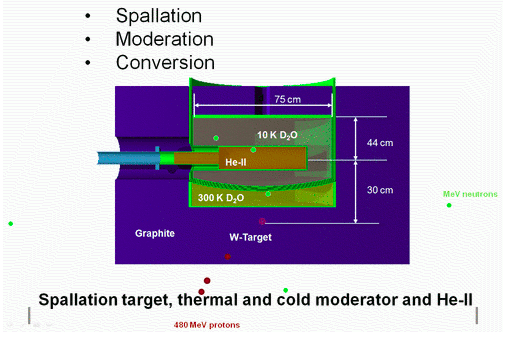
\includegraphics[width=0.9\textwidth]{ucn_production_stages.png}
  \caption{blah}
  \label{fig:ucn_production_stages}
\end{figure}
%\subsection{Neutron Spallation Target}

The neutrons are produced through the spallation process by hitting a
Tungsten target by the proton beam. Spallation is refered to a nuclear
reaction where high energy particles interact with atomic
nucleus. This process creates many high energy neutrons and background
radiation.  The target is surrounded by several blocks of lead and
graphite. These fast neutrons
are reflected and moderated down and enter the warm D$_2$O moderator at room temperature~(300 K) and become thermal
neutrons with an energy of 0.025~eV and the speed of 2.2~km/s.

%\subsection{Neutron Moderation}
Iced heavy water at 20~K is used as a cold moderator. After passing
through the warm D$_2$O, thermal neutrons enter the the cold moderator
and become cold neutrons. These neutrons have the speed of several
hundreds of meter per second.

%\subsection{Neutron Conversion}
The last stage is when the slow neutrons enter the isotopically pure superfluid helium
at 0.84 to 0.92~K. UCN is produced as a result of phonon transitions
inside the superfluid helium as discussed in section~\ref{sec:ucn_with_heII}.


\section{D$_2$O Solidification}
The D$_2$O vessel has a capacity of 100~L. At first, 14~L of liquid
D$_2$O gets injected to the vessel. This is followed by adding 11~L of
D$_2$O to the vessel over 8 times.  After filling up the vessel,
Gifford McMahon refrigerators solidify the heavy water and further
cool it down to 10~K. The process of icing the heavy water takes about
6 days and cooling it down takes another XXX days.

\section{Data Acquisition System}
Here talk about the EPICS and PLC and put pictures. I can also use
stuff from student's reports.

\section{UCN Detectors}
Talk about how each detector works.
\subsection{$^6$He Detector}
\subsection{$^6$Li Detector}



%\begin{description}
%\item{An intro to whatever goes into this chapter}

%\item{Start by showing a nice drawing and then talk about each
 % componet of the facility:}
  
%\item{about proton beam that we get, the magnets and basically how the
%  beam reaches the target and how it looks like (Where can I get this
%  information? Is it written somewhere?)}
  
%\item{A short introduction to say the stages of UCN production and why
%  we need the vertical cryostat (Link to the next stage)}
  
%\item{It also has to be mention that it is the same vertical sourcse
%  as was used at the RCNP and some modifications were made to meet the
%  requirements at triumf. (Where can I find what modifications were
%  made?) Agian this has to be just as a link to the next chapter(maybe?)}
  
%\item{The target and shielding (with pictures?), only a few
%  paragraphs}
  
%\item{Moderation: D2O system (I can use Ryohei's thesis I guess)}
  
%\item{conversion. There is a whole chapter dedicated to the UCN
%  cryogenics. I have to go through details (not too much) of how the
%  cryostat works. I can borrow some infromation from Ryohei's
%  thesis. I am not sure how much of it is related to the next
%  chapter.}
 

%\item{Data acquisition system, epics and plc, I guess there are useful
%  informaion in Sean Vanbergen's report that I can use for this
%  section}
  
%\item{what else?}

%\end{description}
